\chapter{The Ising Model, Mean Field, and the First Phase Transition}

These notes follow Leonard Susskind's ninth lecture on statistical mechanics. The transcript is the primary guide, and the preserved blackboard images from LazyingArt LLC and Video2Book are kept as supporting evidence where the lecture's mathematics is visibly written on the board. The lecture proceeds in a very deliberate order: we first return to the simplest two-state magnet, then solve the one-dimensional Ising model exactly, then ask why higher dimension should behave differently, and finally use mean field to see how a phase transition can appear.

\section{Ising Revisited and One Spin in a Heat Bath}

Susskind begins by correcting the historical record. Ising did not fail to solve the one-dimensional model. He solved it correctly and found no phase transition there. The mistake came later: he generalized that negative result to all dimensions. The whole lecture is aimed at understanding why that extrapolation fails.

To get there, we first reset to the simplest possible subsystem: one spin in equilibrium with the rest of the world. We let
\begin{equation}
\sigma=\pm 1,
\end{equation}
and we write the energy of one spin as
\begin{equation}
E=-j\,\sigma.
\end{equation}
The sign convention is chosen so that positive \(j\) favors the up-spin state.

The one-spin partition function is then
\begin{align}
z &= \sum_{\sigma=\pm 1} e^{-\beta E(\sigma)}
 = \sum_{\sigma=\pm 1} e^{\beta j \sigma} \\
  &= e^{\beta j}+e^{-\beta j}
 = 2\cosh(\beta j).
\end{align}
This is the same two-state system we already know, but now we are viewing it as a subsystem sitting in a heat bath.

The average energy follows from the derivative of \(\log z\):
\begin{align}
\langle E\rangle
  &= -\frac{\partial}{\partial \beta}\log z
   = -\frac{1}{z}\frac{\partial z}{\partial \beta} \\
  &= -j\,\frac{\sinh(\beta j)}{\cosh(\beta j)}
   = -j\,\tanh(\beta j).
\end{align}
Since \(E=-j\,\sigma\), we immediately read off the average spin,
\begin{equation}
\langle \sigma\rangle = \tanh(\beta j).
\end{equation}

At this point the lecture pauses over the graph of \(\tanh(\beta j)\). Its slope at the origin is \(1\); at large positive argument it approaches \(1\); at large negative argument it approaches \(-1\). So low temperature, meaning large \(\beta\), aligns the spin, while very high temperature drives the average spin to zero.

\begin{figure}[ht]
\centering

\includegraphics[width=0.78\textwidth]{lecture_09_figure_02.png}
\caption{One-spin average energy reduced to hyperbolic tangent form. The blackboard chain of equalities is the visual anchor for the calculation of \(\langle E\rangle\).}
\end{figure}

\section{The One-Dimensional Ising Chain and the Real Question}

We now pass from a single magnet to the one-dimensional Ising model. At each site \(i\) sits a spin \(\sigma_i=\pm1\), and the energy of the whole chain is
\begin{equation}
E=-j\sum_i \sigma_i \sigma_{i+1}.
\end{equation}
The minus sign means that parallel neighbors lower the energy. Thus for \(j>0\) the ground states are the two completely aligned configurations: all spins up, or all spins down.

Susskind also notes an important simplification. If we were to change the sign of \(j\), then in one dimension we could redefine every other spin by a sign flip and recover the same mathematics. So the lecture keeps the ferromagnetic sign convention and moves on.

The real physical question is not merely what the Hamiltonian looks like. The question is whether one spin can bias spins arbitrarily far away. The natural diagnostic is the correlation function
\begin{equation}
C(n)=\langle \sigma_i \sigma_{i+n}\rangle.
\end{equation}
If \(C(n)\) remains nonzero as \(n\to\infty\), then the system has long-range memory. If \(C(n)\to0\), then whatever one spin does is eventually forgotten.

This is already the first hint of what magnetization means in the interacting system. Long-range order and long-range memory are two sides of the same coin.

\section{Bond Variables, Factorization, and Correlation Decay}

The lecture now turns to the exact solution of the one-dimensional model. The trick is not to think in terms of the spins themselves, but in terms of the links between neighboring spins. For a finite chain, let us temporarily fix the first spin. Then define the bond variables
\begin{equation}
\mu_i=\sigma_i \sigma_{i+1}.
\end{equation}
Each \(\mu_i\) is again \(\pm1\). If \(\mu_i=+1\), the neighboring spins are parallel; if \(\mu_i=-1\), they are anti-parallel.

Once the first spin is known, the full chain is reconstructed from the bond data. Indeed,
\begin{equation}
\sigma_{i+1}=\sigma_i\,\mu_i,
\end{equation}
and iterating this gives
\begin{equation}
\sigma_{i+n}=\sigma_i\,\mu_i \mu_{i+1}\cdots \mu_{i+n-1}.
\end{equation}
The energy is now simply
\begin{equation}
E=-j\sum_i \mu_i.
\end{equation}
This is the crucial simplification: the interacting chain has been rewritten as a sum over independent bond variables.

Therefore the partition function factorizes:
\begin{align}
Z
&= 2 \sum_{\{\mu_i=\pm1\}} e^{\beta j \sum_i \mu_i} \\
&= 2 \prod_{i=1}^{N-1} \left( \sum_{\mu_i=\pm1} e^{\beta j \mu_i} \right) \\
&= 2\,[2\cosh(\beta j)]^{N-1}.
\end{align}
The outer factor \(2\) comes from the two possible values of the first spin. The exponent \(N-1\) is the number of bonds in a chain of \(N\) spins.

Now the average bond variable is exactly the same computation we did for one spin:
\begin{equation}
\langle \mu_i\rangle=\tanh(\beta j).
\end{equation}
Since \(\mu_i=\sigma_i\sigma_{i+1}\), this is also
\begin{equation}
\langle \sigma_i \sigma_{i+1}\rangle=\tanh(\beta j).
\end{equation}
So nearest neighbors are indeed correlated.

To compute the long-distance correlation, it is best to make the distance convention explicit: from now on, let \(n\) denote the number of bonds between the two spins. Then
\begin{align}
\langle \sigma_i \sigma_{i+n}\rangle
&= \left\langle \mu_i \mu_{i+1}\cdots \mu_{i+n-1}\right\rangle \\
&= \langle \mu_i\rangle \langle \mu_{i+1}\rangle \cdots \langle \mu_{i+n-1}\rangle \\
&= [\tanh(\beta j)]^n.
\end{align}
For every finite temperature, \(|\tanh(\beta j)|<1\). Therefore the correlation decays exponentially with distance.

\subsection{Question \& Answer}

The lecture stops here over a very natural objection.

Why is it legitimate to insert all those intermediate factors when the correlation function is only \(\langle \sigma_i \sigma_{i+n}\rangle\)?

Because we are only inserting factors of \(1\). Between \(\sigma_i\) and \(\sigma_{i+n}\) we insert
\begin{equation}
1=\sigma_{i+1}^2=\sigma_{i+2}^2=\cdots=\sigma_{i+n-1}^2,
\end{equation}
and then regroup the resulting product into neighboring pairs. That is what converts the spin correlation into a product of bond variables. Nothing has been changed; it has only been rewritten in terms of the variables for which the partition function factorizes.

This exact answer matches the lecture's telephone analogy. Each step down the chain costs another factor of \(\tanh(\beta j)\), just as imperfect transmission in a game of telephone eventually destroys the memory of the initial message.

\section{Why Higher Dimension Changes the Story}

At this point the one-dimensional model looks mathematically neat but physically unexciting. It has no phase transition at any finite temperature. Correlations fall away, and long-range memory is lost.

Susskind's pivot is not immediately algebraic. It is conceptual. In one dimension, once one neighbor passes on a wrong message, the next site has no support system. It only hears from one direction. But in two dimensions, or in higher dimensions, a site receives influence from many neighbors. That opens the possibility of something like majority vote, or in modern language error correction. A wrong message can be overruled by the rest.

This is the physical bridge to the next approximation. If one spin has many neighbors, and if the neighbors are already slightly biased, then perhaps what matters is not the precise state of every neighbor but their average effect.

\section{Mean Field in \(d\) Dimensions}

We now move to a \(d\)-dimensional hypercubic lattice. Each spin has \(2d\) nearest neighbors. The lecture emphasizes that the approximation to follow is supposed to be good when \(d\) is large, because then fluctuations among the neighbors are small relative to the average.

For a chosen spin \(\sigma\), the local energy is
\begin{equation}
E_{\text{local}}=-j\,\sigma \sum_{\text{neighbors}} \sigma_{\text{neighbor}}.
\end{equation}

\begin{figure}[ht]
\centering

\includegraphics[width=0.76\textwidth]{lecture_09_figure_03.png}
\caption{The blackboard layout for the mean-field step: a chosen spin in two dimensions, its local interaction energy, and the introduction of the average spin.}
\end{figure}

The board sketch is schematic, but it is useful to redraw the idea cleanly.

\begin{figure}[ht]
\centering
\begin{tikzpicture}[scale=1.2]
\fill (0,0) circle (2pt);
\draw (0,0) -- (1.4,0);
\draw (0,0) -- (-1.4,0);
\draw (0,0) -- (0,1.4);
\draw (0,0) -- (0,-1.4);
\draw (1.4,0) circle (0.08);
\draw (-1.4,0) circle (0.08);
\draw (0,1.4) circle (0.08);
\draw (0,-1.4) circle (0.08);
\node at (0,0.28) {$\sigma$};
\node at (1.85,0) {$\sigma_{\mathrm{neighbor}}$};
\node at (0,1.85) {$\sigma_{\mathrm{neighbor}}$};
\node at (0,-1.85) {$\sigma_{\mathrm{neighbor}}$};
\node at (-2.05,0) {$\sigma_{\mathrm{neighbor}}$};
\end{tikzpicture}
\caption{A clean schematic of one chosen spin and its nearest neighbors in two dimensions.}
\end{figure}

Now suppose the system has an average spin \(\bar{\sigma}\). The mean-field approximation is simply
\begin{equation}
\sum_{\text{neighbors}} \sigma_{\text{neighbor}} \;\longrightarrow\; 2d\,\bar{\sigma}.
\end{equation}
Then the local energy becomes
\begin{equation}
E_{\text{mf}}=-2dj\,\bar{\sigma}\,\sigma.
\end{equation}
This has exactly the same form as the one-spin problem, except that the effective field is now produced by the neighboring spins themselves.

\begin{figure}[ht]
\centering

\includegraphics[width=0.78\textwidth]{lecture_09_figure_04.png}
\caption{The blackboard in mid-substitution: the neighbor sum is being replaced by an effective field proportional to \(2dj\,\bar{\sigma}\).}
\end{figure}

So if we momentarily denote the average of the distinguished spin by \(\bar{\bar{\sigma}}\), then the one-spin formula gives
\begin{equation}
\bar{\bar{\sigma}}=\tanh(2\beta d j\,\bar{\sigma}).
\end{equation}
But translation invariance tells us that the chosen spin is not special. Its average must equal the average of the rest of the lattice. Therefore
\begin{equation}
\bar{\bar{\sigma}}=\bar{\sigma},
\end{equation}
and we obtain the self-consistency equation
\begin{equation}
\bar{\sigma}=\tanh(2\beta d j\,\bar{\sigma}).
\end{equation}

\begin{figure}[ht]
\centering

\includegraphics[width=0.78\textwidth]{lecture_09_figure_05.png}
\caption{The self-consistency equation isolated on the board. The lecture immediately clarifies that \(\bar{\sigma}\) belongs inside the argument of \(\tanh\).}
\end{figure}

\subsection{Question \& Answer}

At this stage the lecture naturally raises a notational question.

Is the final \(\bar{\sigma}\) multiplied outside the hyperbolic tangent, or is it inside the argument?

It is inside the argument. The board spacing is deceptive for a moment, but the spoken lecture makes the point explicitly: this is an implicit equation,
\begin{equation}
\bar{\sigma}=\tanh(2\beta d j\,\bar{\sigma}),
\end{equation}
not a mere proportionality of \(\bar{\sigma}\) to itself.

The lecture also switches notation here: the overbar is being used in place of angle brackets. Thus \(\bar{\sigma}\) and \(\langle \sigma\rangle\) represent the same average spin.

\begin{remark}
The mean-field argument is not being presented as exact for small \(d\). Its justification is that when \(2d\) is large, the average influence of the neighbors dominates their fluctuation. That is why the approximation is introduced only after the lecture has emphasized the importance of many neighbors.
\end{remark}

\section{Self-Consistency, Graphs, and the Phase Transition}

To solve the implicit equation, Susskind makes the simple but effective change of variables
\begin{equation}
y=2\beta d j\,\bar{\sigma}.
\end{equation}
Then the self-consistency equation becomes
\begin{equation}
\frac{y}{2\beta d j}=\tanh y.
\end{equation}

\begin{figure}[ht]
\centering

\includegraphics[width=0.78\textwidth]{lecture_09_figure_06.png}
\caption{The reduced transcendental equation written on the board just before the lecture switches to a graphical solution.}
\end{figure}

This is now perfect for a graphical discussion. The right-hand side is the familiar \(\tanh y\) curve. The left-hand side is a straight line through the origin with slope
\begin{equation}
m=\frac{1}{2\beta d j}.
\end{equation}
At high temperature \(\beta\) is small, so the line is steep. It intersects \(\tanh y\) only at the origin, and therefore \(\bar{\sigma}=0\). That is just the paramagnetic phase.

As we lower the temperature, the slope decreases. The critical moment comes when the line is tangent to \(\tanh y\) at the origin. Since
\begin{equation}
\tanh'(0)=1,
\end{equation}
the critical condition is
\begin{equation}
\frac{1}{2\beta_c d j}=1,
\end{equation}
or equivalently
\begin{equation}
2\beta_c d j=1.
\end{equation}
If we write \(T=1/\beta\), as Susskind eventually does, then in these units
\begin{equation}
T_c=2dj.
\end{equation}
Temperature is being measured in energy units here, which is why this equation compares \(T\) directly with \(j\).

Below the critical temperature the line is shallower than the tangent line, and new nonzero intersections appear. These correspond to nonzero average magnetization.

\begin{figure}[ht]
\centering
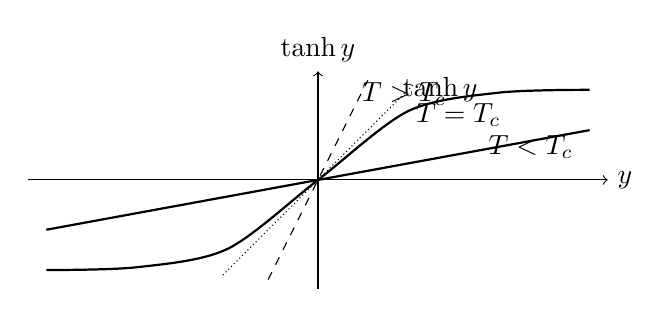
\begin{tikzpicture}[scale=1.15]
\draw[->] (-3.2,0) -- (3.2,0) node[right] {$y$};
\draw[->] (0,-1.2) -- (0,1.2) node[above] {$\tanh y$};

\draw[smooth,thick]
plot coordinates {(-3,-0.995) (-2,-0.964) (-1,-0.762) (0,0) (1,0.762) (2,0.964) (3,0.995)};

\draw[dashed] (-0.55,-1.1) -- (0.55,1.1);
\draw[densely dotted] (-1.05,-1.05) -- (1.05,1.05);
\draw[thick] (-3,-0.55) -- (3,0.55);

\node at (1.35,1.0) {$\tanh y$};
\node at (0.95,0.95) {$T>T_c$};
\node at (1.55,0.72) {$T=T_c$};
\node at (2.35,0.36) {$T<T_c$};
\end{tikzpicture}
\caption{The graphical solution of \(\frac{y}{2\beta d j}=\tanh y\). High temperature gives only the origin, the critical line is tangent there, and lower temperature produces nonzero solutions.}
\end{figure}

There is, however, a tension built directly into the picture. Even below the transition the origin is still an intersection. So why is the magnetized branch the physical one? The lecture does not suppress that question. It turns it into the next step.

\section{Why \(d=1\) Fails, and How a Tiny Field Picks a Branch}

\subsection{Question \& Answer}

What goes wrong if we simply put \(d=1\) into the mean-field equation?

The answer is that the mean-field equation does not know enough about the geometry of low-energy excitations in one dimension. To see the issue, the lecture goes back to very low temperature and asks how much energy it costs to flip spins away from the perfectly aligned ground state.

In one dimension, flipping one spin breaks two bonds. But flipping two adjacent spins still breaks only two bonds. In fact any adjacent block of flipped spins still costs only two broken bonds. Therefore very large domains of reversed spins are entropically cheap: there are many of them, and they do not cost more energy than a tiny reversed domain.

In two dimensions the story changes. Flip one spin and four bonds are broken. Enlarge the reversed region and the energy grows with the boundary of that region. The essential point is that in one dimension the energy cost is tied only to the two endpoints of the domain, while in two dimensions it grows with the size of the domain wall.

This is the missing mathematics behind the failure of long-range order in one dimension at finite temperature. The lecture's low-temperature counting argument may be summarized schematically as follows:
\begin{enumerate}
\item In \(1d\), an adjacent block of any length costs the same two broken bonds.
\item The number of such blocks is large, growing with the choices of their endpoints.
\item Therefore finite temperature immediately populates large flipped domains.
\item In \(2d\), larger droplets cost more energy because their boundary is longer.
\item Therefore large droplets are suppressed much more strongly.
\end{enumerate}

The lecture then returns to the other unresolved question: how a magnetized branch is chosen.

We add a tiny external magnetic field. Choosing the sign convention so that positive \(b\) favors up spins, we write the mean-field energy as
\begin{equation}
E_{\text{mf},b}=-2dj\,\bar{\sigma}\,\sigma-b\,\sigma.
\end{equation}
The one-spin calculation now gives
\begin{equation}
\bar{\sigma}=\tanh(2\beta d j\,\bar{\sigma}+\beta b).
\end{equation}
If we keep the same definition \(y=2\beta d j\,\bar{\sigma}\), this becomes
\begin{equation}
\frac{y}{2\beta d j}=\tanh(y+\beta b).
\end{equation}
So the effect of a nonzero \(b\) is to shift the \(\tanh\) curve. The symmetric origin solution is no longer the relevant one. A tiny field picks one of the two magnetized branches, and if we then let \(b\to0^\pm\), the system remains on that branch. That is the content of spontaneous symmetry breaking in this lecture: the symmetric zero-average state is possible as a formal solution, but it is unstable.

This is why a macroscopic ferromagnet, placed in an arbitrarily small ambient field, does not remain indecisive forever. The smallest bias is enough to choose a direction once the system is below the transition.

\section{Summary}

The lecture begins with a correction to the story of Ising, but it ends with a sharper physical point. One dimension has no phase transition because errors propagate too easily and domain reversals are too cheap. Higher dimensions behave differently because many neighbors support one another, and in sufficiently high dimension a mean-field description becomes plausible.

From the one-spin partition function
\begin{equation}
z=2\cosh(\beta j),
\end{equation}
we inherit the ubiquitous hyperbolic tangent. In one dimension the bond-variable trick makes the model exact and shows
\begin{equation}
\langle \sigma_i \sigma_{i+n}\rangle=[\tanh(\beta j)]^n,
\end{equation}
so correlations decay exponentially. In high dimension mean field replaces the neighbor sum by its average and leads to
\begin{equation}
\bar{\sigma}=\tanh(2\beta d j\,\bar{\sigma}),
\end{equation}
whose graphical solution exhibits a critical temperature and magnetized branches.

That is the lecture's payoff: the Ising model is no longer merely a chain of coupled spins. It becomes the first clear arena in which we can watch long-range order emerge, disappear, and then be selected by the tiniest asymmetry.